\documentclass{report}

\usepackage{tikz}
\usepackage{graphicx}
\usepackage{subcaption}
\usepackage[]{algorithm2e}
\usepackage{algorithmicx}
\usepackage{listings}
\usepackage{url}
\graphicspath{{images/}}

\usetikzlibrary{positioning, arrows, decorations.markings}
\tikzset{%label colors for port states
    port/.style={draw, circle},
    dedicated/.style={port, fill=blue!50},
    root/.style={port, fill=green!50},
    blocking/.style={port, fill=red!50}
}

\tikzset{%used for "invisible" stuff
    invisible/.style={draw=white}
    visible/.style={draw=black}
}

\newcommand{\switch}[2]{
    \scalebox{#1}{
        \begin{tikzpicture}
            \node at (0,0) {
\includegraphics{switch.pdf}};
            \node at (0,-0.6) {#2};
        \end{tikzpicture}
    }
}
\author{Alexander Schloegl, Matr Nr. 1315020}
\title{stp-tree-generator}
\begin{document}
%\raggedright
\lstset{language=C++}
\maketitle
\tableofcontents

\chapter{Introduction}
As networks grow larger and more complex, redundancy becomes desirable and necessary.
With layer 2 (the data link layer in the OSI model, where we have MAC addresses but no IP addresses) redundancy also brings loops and the danger of so called Broadcast Storms (where broadcast messages are bounced back and forth between network nodes).
To this end the Spannning Tree Protocol\cite{perlman85} was created.
Note that the only layer 2 hardware considered in this paper will be Switches, as Hubs are not STP capable and also very rarely used in larger networks.
We will also refer to Switches as Bridges, in order to be compliant with the STP nomenclature\\
The Spanning Tree Protocol (STP) works by creating a logical topology (in the form of a tree) over the physical topology by disabling specific ports.
An example is shown in Figure~\ref{fig:stp_example}

\begin{figure}[h]
    \begin{center}
    \begin{subfigure}[b]{0.4\textwidth}
    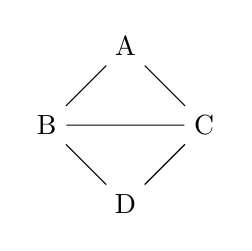
\begin{tikzpicture}
    \node (A) at (2,4) {A};
    \node (B) at (1,3) {B};
    \node (C) at (3,3) {C};
    \node (D) at (2,2) {D};

    \draw
    (A) -- (B)
    (A) -- (C)
    (B) -- (C)
    (B) -- (D)
    (C) -- (D);
    \end{tikzpicture}
    \caption{Physical topology}
    \end{subfigure}
    ~
    \begin{subfigure}[b]{0.4\textwidth}
    \begin{tikzpicture}
    \node (root) at (2,4) {A};
    \node (B) at (1,3) {B};
    \node (C) at (3,3) {C};
    \node (D) at (2,2) {D};

    \draw
    (root) -- (B)
    (root) -- (C)
    (B) -- (D);
    \end{tikzpicture}
    \caption{Logical topology}
    \end{subfigure}
    \end{center}
    \caption{An example of how STP changes the logical network topology}
    \label{fig:stp_example}
\end{figure}

As the networks STP is used in are complex to start with, and as changes and outages are not immediately (if ever) noticed, it can be difficult to keep tabs on the current network layout.
While possible, surveying the results of the STP algorithm via the Simple Network Management Protocol (SNMP) - which many business-grade Bridges are capable of - is tedious and requires the administrator to connect to every single Switch in the Local Area Network (LAN).
The aim of this project and the resulting STP-Tree-Generator (referred to in this paper as the Generator) is to decrease the complexity and workload that this task requires.\\

It achieves this goal by collecting STP packets at different locations in the LAN and then piecing them together at a central server.
The resulting report can then be downloaded from the server.
As of the time of writing this paper, the only output format available is the \LaTeX\ library TikZ.

\chapter{Background}
\label{background}
\section{Existing alternatives}
As of writing this thesis, only very few tools support monitoring of STP topologies.
The ones we found are LoriotPro\cite{LoriotPro}, LiveAction\cite{LiveAction} and L2Discover\cite{L2Discover}.
Of these three network monitoring tools, only L2Discover has its source code openly available.
The company SolarWinds has an open vote on their website on whether or not to include this feature in their monitoring software since 2014\cite{thwackSW}.
LoriotPro and L2Discover use the SNMP for their topology discovery, with STP only being used to discover duplicate and unused links.
\tool\ uses only STP, thus not needing the networking hardware being SNMP capable.

While commercial tools mostly use active methods for network discovery, several research projects have also attempted to develop purely passive or hybrid tools.
One of the first of these tools was developed by Becker et al.\cite{becker1995} in 1995.
In more recent years, Blue et al.\cite{blue2008} and Wongsuphasawat et al.\cite{wongsuphasawat2009} published papers on passive network visualization tools in 2008 and 2009.
However, we did not find any work on using STP exclusively.

\section{Spanning Tree Protocol (STP)}
\label{stp}
\subsection*{Port States}
The most important part of STP is its introduction of port states.
These port states ensure that the spanning tree does not contain loops.
Ports can be in one of three states (see Figure~\ref{fig:port_states}):
\begin{itemize}
    \item \textcolor{green}{\textbf{Root Port}}: the port leading to the root or "upwards" in the tree.
        Every non-root bridge has \textbf{exactly one} root port.
    \item \textcolor{blue!80}{\textbf{Dedicated Port}}: dedicated ports are ports where packets are sent. These are the ports leading "downward" in the tree.
        The root has only dedicated ports.
    \item \textcolor{red}{\textbf{Blocking Port}}: no packets are sent via a blocking Port.
        This state is used to disable alternate paths to the root or "sideways" in the tree.
        In the original paper\cite{perlman85}, this state was called backup.
\end{itemize}
To handle necessary port transitions (e.g. on bridge failure), so called transition states are used.
A blocking port for example waits $forwardDelay$ (see Figure~\ref{fig:stp_bpdu}) seconds in a loop.
Every time a superior BPDU is received, the timer is reset.
If the timer ever hits zero, the port will transition to dedicated.

In the original STP paper\cite{perlman85}, the term Local Area Network (LAN) referred to any connection to a bridge, as well as between bridges.
Because the STP information must be propagated to every LAN, there needs to be exactly one dedicated port in a LAN.
In a LAN between two non-root bridges, the bridge with the smaller root path cost (see Figure~\ref{fig:stp_bpdu}) will make its connected port dedicated.
Should both bridges have the same path cost to the root, the one with the smaller bridge identifier becomes the dedicated bridge (see Section~\ref{stp_packet}: STP Packets).
This can be seen in the connection between the bottom bridges in Figure~\ref{fig:port_states}.
\begin{figure}[h]
    \centering
    \begin{tikzpicture}
        \node (root) at (2,2) {\switch{0.8}{Root}};
        \node (a) at (0,0) {\switch{0.8}{A}};
        \node (b) at (4,0) {\switch{0.8}{B}};

        \draw
        (root) -- node[dedicated, at start]{} node[root, at end]{} (a)
        (root) -- node[dedicated, at start]{} node[root, at end]{} (b)
        (a) -- node[dedicated, at start]{} node[blocking, at end]{} (b);

        \begin{customlegend}[legend cell align=left, legend entries={Root Port,Dedicated Port,Blocking Port},
            legend image post style={scale=2.3},
            legend style={at={(8,2)},font=\footnotesize}]
            \addlegendimage{white,mark=*,fill=green}
            \addlegendimage{white,mark=*,fill=blue!80}
            \addlegendimage{white,mark=*,fill=red}
        \end{customlegend}
    \end{tikzpicture}
    \caption{An example of STP port states}
    \label{fig:port_states}
\end{figure}

\subsection*{STP Packets}
\label{stp_packet}
In this section we will explain the individual fields in an STP Bridge Protocol Data Unit (BPDU), as seen in Figure~\ref{fig:stp_bpdu}.
\begin{figure}[h]
    \centering
    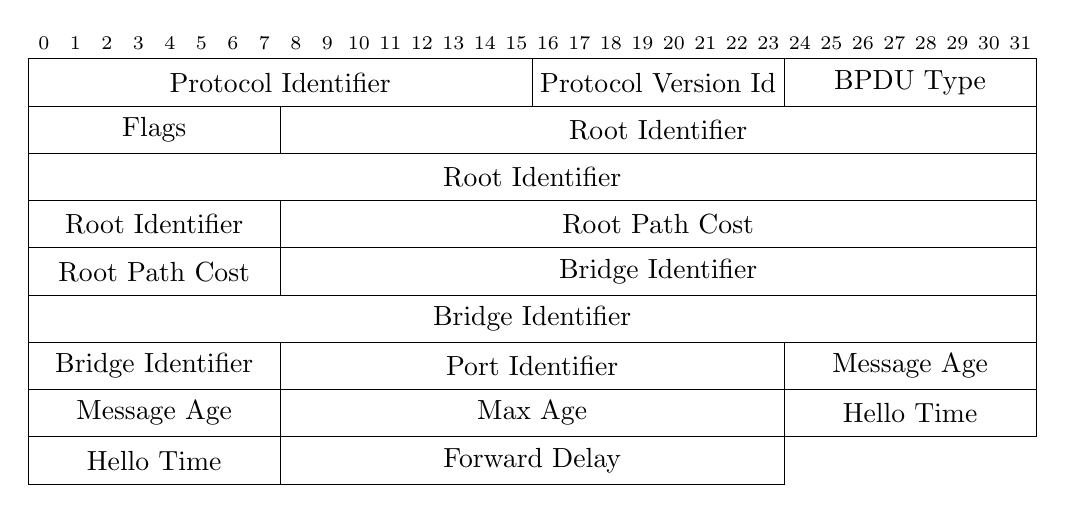
\begin{tikzpicture}[scale=0.4]
        \foreach \x in {0,...,31}
            \node at (\x+0.5,20.5) {\scriptsize \x};
        \draw (0,20) rectangle (16,18.5); \node (mode) at (8, 19.25) {Protocol Identifier};
        \draw (16,20) rectangle (24,18.5); \node (mode) at (20, 19.25) {Protocol Version Id};
        \draw (24,20) rectangle (32,18.5); \node (mode) at (28, 19.25) {BPDU Type};
        \draw (0,18.5) rectangle (8,17); \node (mode) at (4, 17.75) {Flags};
        \draw (8,18.5) rectangle (32,17); \node (mode) at (20, 17.75) {Root Identifier};
        \draw (0,17) rectangle (32,15.5); \node (mode) at (16, 16.25) {Root Identifier};
        \draw (0,15.5) rectangle (8,14); \node (mode) at (4, 14.75) {Root Identifier};
        \draw (8,15.5) rectangle (32,14); \node (mode) at (20, 14.75) {Root Path Cost};
        \draw (0,14) rectangle (8,12.5); \node (mode) at (4, 13.25) {Root Path Cost};
        \draw (8,14) rectangle (32,12.5); \node (mode) at (20, 13.25) {Bridge Identifier};
        \draw (0,12.5) rectangle (32,11); \node (mode) at (16, 11.75) {Bridge Identifier};
        \draw (0,11) rectangle (8,9.5); \node (mode) at (4, 10.25) {Bridge Identifier};
        \draw (8,11) rectangle (24,9.5); \node (mode) at (16, 10.25) {Port Identifier};
        \draw (24,11) rectangle (32,9.5); \node (mode) at (28, 10.25) {Message Age};
        \draw (0,9.5) rectangle (8,8); \node (mode) at (4, 8.75) {Message Age};
        \draw (8,9.5) rectangle (24,8); \node (mode) at (16, 8.75) {Max Age};
        \draw (24,11) rectangle (32,8); \node (mode) at (28, 8.75) {Hello Time};
        \draw (0,8) rectangle (8,6.5); \node (mode) at (4, 7.25) {Hello Time};
        \draw (8,8) rectangle (24,6.5); \node (mode) at (16, 7.25) {Forward Delay};
    \end{tikzpicture}
    \caption{An STP BPDU}
    \label{fig:stp_bpdu}
\end{figure}\\
The fields we used for \tool\ are:
\begin{itemize}
    \item \textbf{Flags}: The flags byte is used for the \textit{topology change (TC)} and \textit{topology change acknowledgement (TCA)} flags.
    \item \textbf{Root/Bridge Identifier}: The Identifier consists of three parts and has the same layout for the root and regular bridges:
        \begin{itemize}
            \item Priority (4 Bits): A value between 0 and 61440 configurable in increments of 4096
            \item System ID Extension (12 Bits): Used for keeping the bridge ID unique if multiple VLANs are configured for a bridge
            \item Bridge MAC (6 Bytes): The MAC address of the bridge
        \end{itemize}
        The conjunction of these three parts is used in comparisons as one large eight byte number.
        \item \textbf{Root Path Cost}: The root path cost is the sum of all port costs along the current path.
            Port Cost can be configured manually or detected automatically.
            The root path cost in packets sent by the root is zero.
    \item \textbf{Message Age}: The message age is the number of bridges that have been passed (in addition to the root) along the current path.
    \item \textbf{Max Age}: If the message age surpasses this maximum, packages are not forwarded any more.
    \item \textbf{Hello Time}: The delay in seconds between sent \textit{Hello} BPDUs.
        \textit{Hello} BPDUs have the form shown in Figure~\ref{fig:stp_bpdu}.
    \item \textbf{Forward Delay}: After this time, if no superior packet was received, a root, or blocking port will transition to dedicated.
        Note that if a root port transitions to dedicated state due to timeout, the bridge now assumes it is the root.
\end{itemize}
A BPDU only contains information about the root and the bridge that sent the package.
This means that if there is a bridge between these two, we will not know about its ID.
We will however still know that it is there, because of the message age.
During the buildup of the tree it is possible to obtain information on intermediate nodes.
This possibility is explained more in-depth in the section on packet handling (Section~\ref{packet_handling}).

\subsubsection*{Default Parameters}
Unless otherwise conifgured the parameters discussed default to the following values\cite{params}:
\begin{itemize}
    \item \textbf{Priority}: 32768
    \item \textbf{System Id Extension}: 0
    \item \textbf{Max Age}: 20
    \item \textbf{Forward Delay}: 15
    \item \textbf{Hello Time}: 2
\end{itemize}

\subsection*{Spanning Tree Algorithm}
The original paper on STP does not describe an algorithm itself, it merely lists constraints that have to be fulfilled.
Algorithm~\ref{alg:stp} shows the algorithm we use in our own \textit{software-switch} testing tool.
We use a reduced number of port states, ignoring the transition states, by utilizing the timestamps of received BPDUs.
The algorithm's purpose is to keep loops out of the network, as well as keeping the tree topology consistent.

\begin{algorithm}[h]
    \DontPrintSemicolon
    \KwData{\\
    $received$ = received packet\;
    $current$ = data of the current bridge\;
    }
    \;
    \If{$received.rootId < current.rootId$}{
        \tcc{There is a new root in the network}
        $current.rootId=other.rootId$\;
        set receiving port as root-port\;
        set other ports to dedicated\;
    }{
        \uIf{$received.rootPathCost<current.rootPathCost$}{
            \tcc{This means that the path via the other bridge is shorter, so this should be our new root-path}
            set receiving port as root-port\;
            set other ports to dedicated\;
        }
        \ElseIf{$received.rootPathCost==current.rootPathCost \land received.bridgeId<current.bridgeId$}{
            \tcc{Both bridges are equidistant from the root, but the other bridge has a lower bridge Identifier and should be the dedicated bridge on the connection}
            set receiving port as blocking port\;
        }
        \tcc{Check if the transitions described in the section on \textbf{STP Packets} are necessary}
        doPacketTimeOutTransitions()\;
    }
    
    \caption{Spanning Tree Algorithm (STA)}
    \label{alg:stp}
\end{algorithm}

\subsection*{Extensions}
Since the inclusion of STP in the IEEE 802.1D\cite{802.1D} standard, multiple additions have been made to the STP.
Rapid STP (RSTP) has been developed to decrease the time needed for tree convergence.
Per VLAN STP (PVSTP) has been developed by Cisco and is a proprietary variant which allows for multiple spanning trees to exist, one for each VLAN.
The Multiple STP (MSTP) is an extension of RSTP which, like PVSTP, allows for multiple spanning trees to exist in their own VLAN.
In addition to that, it also allows for VLAN specific trees to be combined into one large spanning tree.

As an extension to STP the Shortest Path Bridging (SPB)\cite{spb} protocol was developed.
It allows for multiple paths to be active at the same time, and uses global information to allow for the calculation of shortest paths.

While the aforementioned extensions to STP would make our task a lot easier (especially SPB), they are not as prevalent as basic STP (which most switches are capable of).
For this reason we decided to confine our efforts to basic STP.

\section{Technologies used}
\subsection*{PCAP}
\label{pcap}
PCAP\cite{pcap} is a shortening of packet capture.
It used to be a part of the \textit{tcpdump} tool before it was moved to its own library.
We used the UNIX version \textit{libpcap} for this thesis.
\textit{Libpcap} is a C library and can be directly linked with C and C++ without using a wrapper.
It provides functions for opening live network devices and \textit{.pcapng} files.
After starting a live capture on a device, \textit{libpcap} will call a callback function for every packet received on the opened interface.
The prototype of the callback function looks as follows:
\begin{lstlisting}[caption=Pcap Callback Prototype]
typedef void (*pcap_handler)(u_char *user, const struct pcap_pkthdr *h, const u_char *bytes);
\end{lstlisting}
Where the parameters are:
\begin{itemize}
    \item \textbf{u\_char *user} is used to pass user defined parameters.
    \item \textbf{pcap\_pkthdr *h} contains useful information about the packet, like source and destination addresses, as well as size.
    \item \textbf{u\_char *bytes} contains the actual (binary) data of the packet.
\end{itemize}
The \textbf{typedef void} (*pcap\_handler) part of the prototype just means that the function returns a \textbf{void *}.

Usage of this function will be covered more in-depth in the chapter on \tool\ itself (Chapter~\ref{stp-gen}).
\subsection*{JSON}
\label{json}
JSON stands for Java Script Object Notation and was used for two reasons:
\begin{enumerate}
    \item It keeps the network communication independent from any programming languages used.
    \item Utility libraries for JSON are easily available for most programming and scripting languages, saving us the work of inventing and implementing our own notation.
\end{enumerate}
JSON has a simple notation for declaring objects and arrays, as well as primitive data types.
An example is shown in Listing~\ref{lst:json}.
\lstinputlisting[caption=JSON Example, label=lst:json]{../listings/json/example.json}
The JSON library used in this thesis is \textit{jsoncpp}\cite{jsoncpp}.

\subsection*{TikZ}
\label{tikz}
We chose TikZ ist kein Zeichenprogramm (TikZ)\cite{tikz} as the file format for our output.
Using TikZ allows us to generate \textit{.tex} files rather than images.
These are easier to generate, as well as to modify after creation.
They are also very easy to integrate in \LaTeX\ papers.
While TikZ is very powerful and therefore complex, the parts we use are fairly simple.
Listing~\ref{lst:tikz_example} shows the TikZ code for Figure~\ref{fig:bc_storm_b}.
\lstinputlisting[caption=A TikZ Example, label=lst:tikz_example]{../listings/tikzExample.tex}
The \textbackslash node keyword draws a node with the id given in parenthesis.
It is centered around the coordinates given with the \textit{at} keyword and has the text written in braces.
The (0,0) coordinate is in the top left corner of an image.
For our graphics we used a self defined \textbackslash switch macro, but regular text or \LaTeX\ commands work as well.
Edges are drawn using the \textbackslash draw command.
This command can be used with raw coordinates or identifiers.
Options for the edges can be passed in brackets.
Note that \textit{edge} can be substituded with \textit{- -}.
All TikZ commands are ended with a semicolon.
TikZ graphics are automatically cropped on rendering.


\chapter{STP Tree Generator}
\label{stp_gen}
\section{Structure}
We split the application in three parts:
\begin{itemize}
    \item \textbf{Client}: collects STP information and sends it to the server.
        The client also handles piecing together the packets into paths.
    \item \textbf{Server}: saves the data from the clients and combines them into one tree.
    \item \textbf{Parser}: contacts the server to receive the tree and converts it into output format.
\end{itemize}
The intended form of usage is to have multiple clients in the network connecting to one server.
This naturally increases the amount of information obtainable.
STP uses only local data, which means that bridges have no knowledge of the network, except for their own port states.
Unfortunately for us, this means that it is hard to find connections between bridges.
The only way to obtain this information is to capture packets during the tree build up.
Because bridges use the default parameters they use (see Section~\ref{stp}), they will think of themselves as root.
Therefore they will propagate this information, which we can then capture.
Using the root identifier in conjunction with the message age, we can gain information about the tree structure.
An explanation of this can be found in Figures \ref{fig:build_up} and \ref{fig:information_loss}.
\begin{figure}
    \begin{centering}
        \begin{subfigure}[b]{0.4\textwidth}
            \begin{tikzpicture}
                \node (a) at (4,4) {\switch{0.8}{A}};
                \node (b) at (4,2) {\switch{0.8}{B}};
                \node (client) at (4,0) {Client};

                \draw
                (a) -- node [left] {root: A} ++ (b);

                \draw[green, thick, ->]
                (b) -- node [left] {root: B} ++ (client);

            \end{tikzpicture}
            \caption{B thinks it is root}
        \end{subfigure}
        \hspace{1cm}
        \begin{subfigure}[b]{0.4\textwidth}
            \centering
            \begin{tikzpicture}
                \node (a) at (4,4) {\switch{0.8}{A}};
                \node (b) at (4,2) {\switch{0.8}{B}};
                \node (client) at (4,0) {Client};

                \draw[green, thick]
                (a) -- node [right] {root: A} ++ (b);
                \draw[green, thick, ->]
                (b) -- node [right] {root: A} ++ (client);
            \end{tikzpicture}
            \caption{Root information updated}
        \end{subfigure}
    \end{centering}
    \caption{Information gained on STP build up}
    \label{fig:build_up}
\end{figure}
\begin{figure}
    \begin{centering}
        \begin{subfigure}[b]{0.4\textwidth}
            \begin{tikzpicture}
                \node (a) at (4,6) {\switch{0.8}{A}};
                \node (b) at (2,4) {\switch{0.8}{B}};
                \node (c) at (6,4) {\switch{0.8}{C}};
                \node (d) at (4,2) {\switch{0.8}{D}};
                \node (client) at (4,0) {Client};
                \draw
                (a) -- (c)
                (c) -- (d);
                \draw[green, thick]
                (b) -- node [left] {root: B} ++ (d)
                (d) -- node [left] {root: B} ++ (client);
            \end{tikzpicture}
            \caption{Some information known}
        \end{subfigure}
        \hspace{1cm}
        \begin{subfigure}[b]{0.4\textwidth}
            \begin{tikzpicture}
                \node (a) at (4,6) {\switch{0.8}{A}};
                \node (b) at (2,4) {\switch{0.8}{B}};
                \node (c) at (6,4) {\switch{0.8}{C}};
                \node (d) at (4,2) {\switch{0.8}{D}};
                \node (client) at (4,0) {Client};
                \draw
                (b) -- (d);
                \draw[green, thick]
                (d) -- node [right] {root: A} ++ (client);
                \draw[red, thick]
                (c) -- node [right] {root: A} ++ (d)
                (a) -- node [right] {root: A} ++ (c);
            \end{tikzpicture}
            \caption{Previous information lost}
        \end{subfigure}
        \caption{Information lost during tree build up}
    \end{centering}
\end{figure}
Unfortunately, this works only if the message age increases by one.
If any other change occurs, the client has to clear its data.
This is because in these cases we cannot guarantee that no other changes occured.
More on this can be found in the section on packet handling (Section~\ref{packet_handling}).

\section{Communication}
\section{Details}
\section{Installation \& Usage}

\chapter{Software Switch Testing Utility}
\label{switch}
The original plan for testing the tool was to use cheap routers running \textit{OpenWrt}\cite{OpenWrt} with STP enabled.
This did not work for multiple reasons.
\begin{itemize}
    \item \textit{OpenWrt} routers handle the internal switch as one interface, which stops it from disabling single switch ports.
    \item Through testing we found that the packets sent by the \textit{OpenWrt} implementation are not recognized by our other devices.
    The other devices were a \textit{TP-Link TL-SG2008 Gigabit Smart Switch} and an \textit{ASUS RT-N56U Wireless Router}.
    These two devices would just forward the \textit{OpenWrt} STP packets while still sending their own.
    \item We also found that \textit{OpenWrt} just forwards received STP packets, without appending its own data.
    This alone would make it unusable for our purposes.
\end{itemize}

After making these discoveries, we tried \textit{dd-wrt}\cite{dd-wrt} as an alternative.
Unfortunately, it shares the same behaviour with \textit{OpenWrt} and we did not know whether or not we could make either of these operating systems work for this project.

In order to be able to stay within the time limit while still testing our tool, we decided to implement a bridge capable of STP.
It uses \textit{pcap} to handle incoming packets and react to STP packets.
Our \textit{software-switch} can be run on any number of interfaces, however, it has not been tested on more than two.
The source code for the \textit{software-switch} can be found in its git\cite{soft-switch}.
It was written in C, in contrast to the \textit{stp-tree-generator} which was written in C++.

\section{Saving Switching Data}
\lstinputlisting[caption=The Containers for Switching Data, label=lst:switchData]{../listings/switch/data.c}
Listing~\ref{lst:switchData} shows the variables and arrays we use for saving the switching data.
The \textit{names}, \textit{neighbours} and \textit{interfaces} arrays are arrays of "strings".
They store the local interface names (as returned by the \textit{ifconfig} command), the connected MAC addresses and the local MAC addresses respectively.
As basic C does not have strings, these are arrays of \textbf{char} arrays.
In C, arrays are saved as pointers to the first element, with the other elements following sequentially after that.
This makes \textit{names}, \textit{neighbours} and \textit{interfaces} pointers to pointers.
Because the \textit{software-switch} can be run on multiple interfaces we need to keep track of the number of interfaces it is running on, which we do in \textit{n}.
To know which interface to forward a packet on, switches keep a so-called MAC table.
We keep a list of MAC addresses for every interface, making \textit{macTable} an array of arrays of \textbf{char} arrays.
This is due to us saving MAC adrresses as \textbf{char} arrays as well.

The \textit{ifaceMutex} variable (mutex stands for mutual exclusion) is used to synchronize our different threads.
We use two threads per interface.
One to handle and forward incoming packets, as well as update our STP port states.
The other one sends the STP packets every $helloTime$ seconds.
Sharing memory between \textit{pthreads} (the C thread implementation we used) does not require any setup, as all heap memory is shared\cite{pthreads}.
We need to synchronize these accesses to keep the different threads from corrupting data due to concurrent writes.

\section{Handling STP Packets and Port States}
The code that handles STP packets is almost identical to the main tool.
Extraction of the values stays exactly the same, as packets have the same format.
Handling of this data is a lot different from the \textit{stp-tree-generator}.
The code for this can be found in Listing~\ref{lst:portStates}.
Parameters prefixed with \textit{r} or \textit{b} are gained from the incoming packet and stand for root and bridge (first hop) respectively.
Values prefixed with \textit{root} are for the root information currently saved in the bridge.
\textit{CurrentIndex} is the index of the interface the packet was received on.
\lstinputlisting[caption=Updating Port States, label=lst:portStates]{../listings/switch/portStates.c}

\section{Handling Non STP Packets}
Non STP packets are forwarded based on port states and knowledge of the target MAC address.
We did not implement any special handling for broadcast messages.
None of the packets that the bridge receives should ever come from a broadcast address, which means they should never be contained in the MAC table.
As packets to unknown MAC addresses are broadcast by default, we do not need special behaviour.
\lstinputlisting[caption=Handling Non-STP Packets, label=lst:nonStp]{../listings/switch/forwarding.c}

\section{Installation and usage}
This utility tool was written in C99.
While only one build target exists, we included a Makefile for convenience.
The \textit{pcap} development library is required to compile, and the regular \textit{pcap} library is needed on launch.
Following parameters can be set on launch:
\begin{itemize}
    \item \textbf{-p} sets the STP priority (default: 0x80).
    \item \textbf{-e} sets the system id extension (default: 0).
    \item \textbf{-ms} sets the number of MAC addresses to store per interface (default: 30).
\end{itemize}
After these optional parameters the names of the interfaces to bridge are expected.
The parameters used are printed to \textbf{stdout} for debugging purposes.
Information on STP packets sent, including the respective port states is printed to \textbf{stdout} as well.

\chapter{Testing}
\section{Setup}
The original paper discussing STP is openly available.
However, it does not dictate exact implementation details.
Therefore, in order to reach an accurate enough understanding of it multiple tests were performed.
To minimize external influences these tests needed to be done in a network disconnected from any external network.
Additionally, to be able to check the results for correctness, we kept the network small and simple.
The layout of the test setup can be seen in Figure~\ref{fig:test_setup}.
While a very basic network, it is sufficient for the tests described below, which will guarantee the required capabilities of the developed tool.
The root in figure~\ref{fig:test_setup} was made root by manually assigning it a higher priority than the other bridges (note that \textit{higher} in this case means \textit{smaller}).
Bridges \textit{A}, \textit{B} and \textit{C} had their priorities left to the default value.
Nodes \textit{A}, \textit{B} and \textit{C} were running \textit{Wireshark} and the developed tool.
Additionally using \textit{Wireshark} allowed us to check the actual packages involved in the testing process to monitor progress and note situations not handled correctly by the tool.
The server for our tool was run on Node \textit{A}.
Test results were checked for their correctness by checking the report provided by the tool.

\begin{figure}[h]
    \centering
    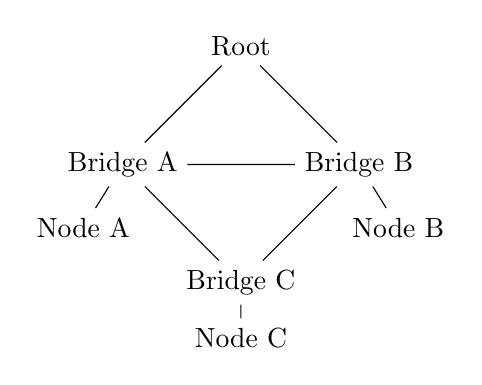
\begin{tikzpicture}
    \node (root) at (2, 4) {Root};
    \node (a) at (0.5, 2.5) {Bridge A};
    \node (na) at (0, 1.7) {Node A};
    \node (b) at (3.5, 2.5) {Bridge B};
    \node (nb) at (4, 1.7) {Node B};
    \node (c) at (2, 1) {Bridge C};
    \node (nc) at (2, 0.3) {Node C};
    \draw 
    (root) -- (a)
    (root) -- (b)
    (a) -- (b)
    (a) -- (b)
    (a) -- (c)
    (b) -- (c)
    (a) -- (na)
    (b) -- (nb)
    (c) -- (nc);
    \end{tikzpicture}
    \caption{Test setup}
    \label{fig:test_setup}
\end{figure}

\section{Tests}
\subsection{Usage Test}
\label{usage_test}
The Usage test proves the general capability of the tool.
It is designed to simulate the connection of nodes to an established network.
Using a simple setup like shown in Figure~\ref{fig:test_setup} allows us to collect information about the whole network.
If the spanning tree were more than 2 layers deep and we were using less nodes than bridges in the network some information about the topology would be unobtainable without additional information.

\subsubsection{Performing the test}
\begin{enumerate}
    \item The layout shown in Figure~\ref{fig:test_setup} was established and all devices were started.
    \item No tool was started yet, identification during the tree establishment is covered by the Tree Establishment Test (\ref{tree_est_test})
    \item We waited for the bridges to establish a stable spanning tree, checking the progress by observing the STP packets for the TC flag.
    \item After the tree had stabilized we started the server on node \textit{A} and the tools on all the nodes.
    \item We waited for the tools to send their data to the server, which takes one $helloTime$ plus the latency between the nodes and the server. Default value for the $helloTime$ is 2 seconds.
    \item When all nodes had sent their data to the server we created a report to check it against the expected result.
\end{enumerate}
\subsubsection{Expected Result}
With the limited size of the test network all bridges can and must be identified correctly for this test to be counted as successful.

\subsection{Tree Establishment Test}
\label{tree_est_test}
To test whether the tool can handle bridges being added to the network during runtime, we start the tool on all nodes before the establishment of the spanning tree, and check for correct identification afterwards.

\subsubsection{Performing the test}
\begin{enumerate}
    \item The layout shown in Figure~\ref{fig:test_setup} was established and all devices were started.
    \item Before enabling STP on all the bridges we started the server and tools.
    \item After enabling STP on the bridges we waited for the tree to be established, again checking the progress via the TC flag.
    \item Lastly we checked the result for correctness.
\end{enumerate}

\subsubsection{Expected Result}
Again all the bridges can and must be correctly identified.

\subsection{Bridge Removal Test}
\label{removal_test}
The tool must also be able to handle bridges dropping from a network.
This test makes sure that capability is given.

\subsubsection{Performing the test}
\begin{enumerate}
    \item We started all the nodes and tools and waited for the spanning tree to be established and correctly identified (see the sections on the Usage Test \ref{usage_test} and the Tree Establishment Test \ref{tree_est_test}).
    \item After the tree was constructed we unplugged Node \textit{B} and waited for the tree to stabilize.
    \item Finally we checked the output of the report for correct identification of the smaller tree.
\end{enumerate}

\subsubsection{Expected Result}
The new path through which Node \textit{C} is connected to the root must be correctly identified.

\subsection{Slow Dynamic Change Test}
\label{slow_dynamic_test}
Changes in the network topology must not be a problem for the tool.
By successfully testing for additions and removals from the network (sections \ref{usage_test} and \ref{removal_test}) one could assume that changes can be handled as well, but caution demands that we test specifically for changes in the topology.
Node \textit{C} is connected to the root either via node \textit{A} or node \textit{B}.
The node with the smaller MAC address (as they have the same priority) will be the preferred hop on the path to the root.
Therefore the logical topology will look like either one of the figures in Figure~\ref{fig:possible_topologies}.
In our case bridge \textit{C} was logically connected to bridge \textit{A} as that was the possible connection to the root with the smaller MAC address.

\begin{figure}[hp]
    \centering
    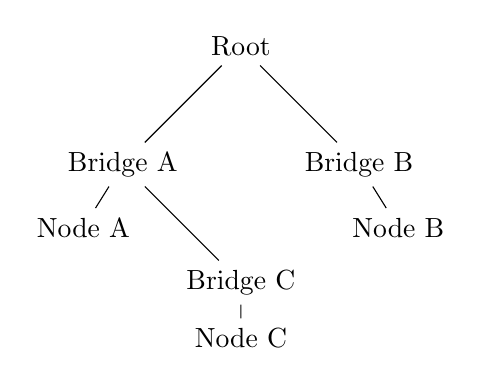
\begin{tikzpicture}
    \node (root) at (2, 4) {Root};
    \node (a) at (0.5, 2.5) {Bridge A};
    \node (na) at (0, 1.7) {Node A};
    \node (b) at (3.5, 2.5) {Bridge B};
    \node (nb) at (4, 1.7) {Node B};
    \node (c) at (2, 1) {Bridge C};
    \node (nc) at (2, 0.3) {Node C};
    \draw 
    (root) -- (a)
    (root) -- (b)
    (a) -- (c)
    (a) -- (na)
    (b) -- (nb)
    (c) -- (nc);
    \end{tikzpicture}
    \hspace{1cm}
    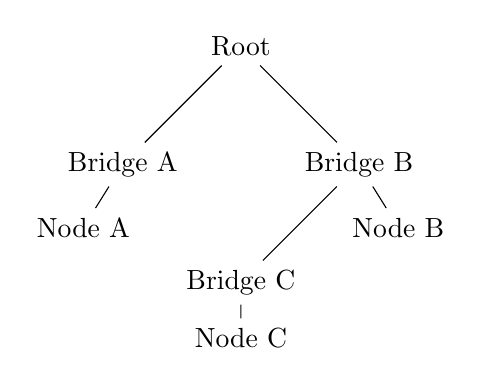
\begin{tikzpicture}
    \node (root) at (2, 4) {Root};
    \node (a) at (0.5, 2.5) {Bridge A};
    \node (na) at (0, 1.7) {Node A};
    \node (b) at (3.5, 2.5) {Bridge B};
    \node (nb) at (4, 1.7) {Node B};
    \node (c) at (2, 1) {Bridge C};
    \node (nc) at (2, 0.3) {Node C};
    \draw 
    (root) -- (a)
    (root) -- (b)
    (b) -- (c)
    (a) -- (na)
    (b) -- (nb)
    (c) -- (nc);
    \end{tikzpicture}
    \caption{The 2 possible paths to the root from node \textit{C}}
    \label{fig:possible_topologies}
\end{figure}

\subsubsection{Performing the test}
\begin{enumerate}
    \item We set up all the nodes and waited for a stable tree to be generated by the bridges like before (sections \ref{usage_test}, \ref{tree_est_test} and \ref{removal_test}).
    \item We disconnected bridge \textit{A} from the root, leaving us with a 2 bridge subtree.
    \item The connection between bridges \textit{A} and \textit{B} was also severed, as well as the connection between bridge \textit{C} and \textit{B}.
    \item We waited for the spanning tree to stabilize after the removal.
    \item Bridges \textit{A} and \textit{C} were connected to bridge \textit{B} yielding the physical topology shown in Figure~\ref{fig:deep_topology}.
    \item After the tree had stabilized we checked the report output for correctness.
\end{enumerate}

\begin{figure}[hp]
    \centering
    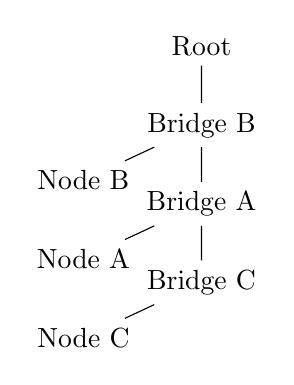
\begin{tikzpicture}
    \node (root) at (2, 4) {Root};
    \node (b) at (2, 3) {Bridge B};
    \node (nb) at (0.5, 2.3) {Node B};
    \node (a) at (2, 2) {Bridge A};
    \node (na) at (0.5, 1.3) {Node A};
    \node (c) at (2, 1) {Bridge C};
    \node (nc) at (0.5, 0.3) {Node C};
    \draw 
    (root) -- (b)
    (b) -- (a)
    (a) -- (c)
    (a) -- (na)
    (b) -- (nb)
    (c) -- (nc);
    \end{tikzpicture}
    \caption{The physical network after performing the steps described in the Slow Dynamic Change Test \ref{slow_dynamic_test}}
    \label{fig:deep_topology}
\end{figure}

\subsubsection{Expected Result}
The tool must correctly identify the new topology.

\subsection{Fast Dynamic Change Test}
\label{fast_dynamic_test}
Robustness to changes in the topology are a must for the developed tool.
It would however also be nice if the tool were robust enough to handle topology changes without a spanning tree stabilization in between.
The logical topology is the same as for the Slow Dynamic Change Test \ref{slow_dynamic_test}

\subsubsection{Performing the test}
\begin{enumerate}
    \item We set up all the nodes and waited for a stable spanning tree.
    \item After we removed node \textit{A} from the network we immediately plugged nodes \textit{A} and \textit{C} into B.
    \item We waited $2*helloTime$ to make sure the changes were propagated to the server before plugging node \textit{C} into the root.
    \item Finally we waited for the tree to stabilize and checked the output for correctness.
\end{enumerate}

\subsubsection{Expected Result}
Whether the output was correct or not gave us information about the capabilities of the tool.
Due to its distributed nature it is also difficult to debug and this gave us additional insights into the execution behavior.

\chapter{Conclusion}
Gaining information about bridges in the network is easy.
Gaining information about the connections in between is a lot harder, and only possible under certain conditions.
By observing changes to the packets sent during buildup of the spanning tree, we can the tree has a certain shape.
These assumptions, however, are not correct in every case.
We can only try to minimize these errors by combining data sent from multiple clients.
This means that the usefulness of the tool discussed increases greatly with the number of clients running on a network.
Unfortunately we did not find any other general method of checking assumed topologies.
The lack of mechanics like a hop count on the Data Link layer keeps us from implementing something like a \textit{traceroute}, which we could use to check our assumptions manually.

Future extensions of this tool could include features to increase usability, like a GUI, as well as other output formats.
The \textit{README} in the git should also be extended to include the parts of this thesis paper that are vital to using the tool.
Additionally we should extend the parser to be capable of generating output from one or more \textit{.pcapng} files without needing to launch a server and multiple clients beforehand.
Our approach to handling network topology changes could also be improved.
With more extensive testing and statistical analysis of the results, it is our opininon that the assumptions we make can be greatly improved.

The \textit{software-switch} utility could also be extended and tested, in order to make it usable as a general purpose switching utility.
Other extensions of this thesis include work on the \textit{OpenWrt} and \textit{dd-wrt} projects in order to find a viable method to keep the STP implementation consistent with other hardware.


\bibliographystyle{plain}
\bibliography{sources}
\end{document}
